\documentclass[12pt]{jarticle}
\usepackage{TUSIreport}
\usepackage{otf}
\usepackage[dvipdfmx]{graphicx}
\usepackage[dvipdfmx]{color}
\usepackage{amsmath}
\usepackage{amssymb}
\usepackage{color}
\usepackage{hhline}
\usepackage{fancybox,ascmac}
\usepackage{multirow}
\usepackage{url}
\usepackage{bm}
\usepackage{listings,jlisting}
%%%%%%%%%%%%%%%%%%
\lstdefinestyle{py}{
    language={Python},
    backgroundcolor={\color[gray]{.85}},
    basicstyle={\small},
    identifierstyle={\small},
    commentstyle={\small\ttfamily \color[rgb]{0,0.5,0}},
    keywordstyle={\small\bfseries \color[rgb]{1,0,0}},
    ndkeywordstyle={\small},
    stringstyle={\small\ttfamily \color[rgb]{0,0,1}},
    frame={tb},
    breaklines=true,
    columns=[l]{fullflexible},
    numbers=left,
    xrightmargin=0zw,
    xleftmargin=3zw,
    numberstyle={\scriptsize},
    stepnumber=1,
    numbersep=1zw,
    morecomment=[l]{//}
}
\begin{document}
%%%%%%%%%%%%%%%%%%%%%%%%%%%%%%%%%%%%%%%%%%%%%%%%%%%%%%%%
% 表紙を出力する場合は,\提出者と\共同実験者をいれる
% \提出者{科目名}{課題名}{提出年}{提出月}{提出日}{学籍番号}{氏名}
% \共同実験者{一人目}{二人目}{..}{..}{..}{..}{..}{八人目}
%%%%%%%%%%%%%%%%%%%%%%%%%%%%%%%%%%%%%%%%%%%%%%%%%%%%%%%
\提出者{情報工学実験3}{課題4 画像変換}
{2021}{4}{22}{4619055}{辰川力駆}
%%%%%%%%%%%%%%%%%%%%%%%%%%%%%%%%%%%%%%%%%%%%%%%%%%%%%%%%%
\共同実験者{}{}{}{}{}{}{}{}
%%%%%%%%%%%%%%%%%%%%%%%%%%%%%%%%%%%%%%%%%%%%%%%%%%%%%%%%%
% 表紙を出力する場合はコメントアウトしない
%%%%%%%%%%%%%%%%%%%%%%%%%%%%%%%%%%%%%%%%%%%%%%%%%%%%%%%%%
\表紙出力
%%%%%%%%%%%%%%%%%%%%%%%%%%%%%%%%%%%%%%%%%%%%%%%%%%%%%%%
% 以下はレポート本体,reportmain.tex に書いてある.
% \inputを使っているが,直接書いても良い.
%%%%%%%%%%%%%%%%%%%%%%%%%%%%%%%%%%%%%%%%%%%%%%%%%%%%%%%
\section{実験の要旨}

実験環境を整備した上で、
Jupyther notebookでPython言語とそのライブラリの使い方を理解し、
画像処理の基礎を学習する。

\section{実験の目的}

画像変換の処理を題材に、
画像処理のプログラミングと評価を通じて、
画像処理の基本的な考え方を理解することを目的とする。

第1回目の実験では、濃淡変換の実装と実験を通じて、
Python言語とライブラリの使用方法、
画像処理の基本を理解することを目的とする。

\section{課題1}
\subsection{実験方法}
次のようなプログラムを作成する。
ただし、指定の領域は、2点(64,25),(192,220)を対角とする矩形である。
\begin{enumerate}
    \item 画像ファイル data/Mandrill.bmp を読み込み画像im1とする。
    \item 画像im1の指定の領域をグレースケールにした画像im2を作成する。
    \item 画像im1の指定の領域を上下反転した画像im3を作成する。
    \item 画像im1、im2、im3にタイトルを付けて、横に並べて表示する。
\end{enumerate}

\subsection{実験結果}

作成したプログラムは付録のソースコード1に載せた。
このプログラムを実行すると、
以下のようになった。

\begin{figure}[h]
    \begin{center}
        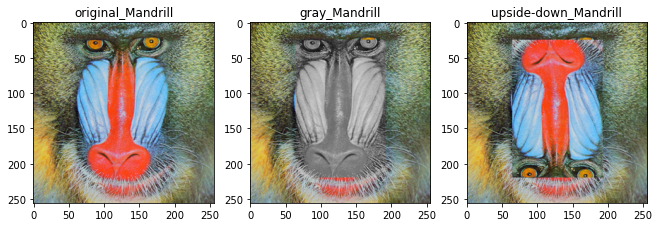
\includegraphics[scale=0.7]{kadai4_1_1.png}
    \end{center}
    \caption{課題1の実行結果}
\end{figure}

\subsection{検討・考察}

im1の一部を反転させるのは、容易であったが(upside-down\_Mandrill)、
im1の一部をグレースケールにするには、
一点一点を変更していく(プログラム11行目から13行目)ので、
高速に実行するのは難しいと考える。

\section{課題2}
\subsection{実験方法}
自分自身で撮影した画像$f$に対して、以下を実行する。
\begin{enumerate}
    \item ガンマ値$\gamma$を変化させながら、画像$f$にガンマ補正を施した結果を求める。
    \item ガンマ補正によるコントラスト向上の効果を確認する。そして、見た目が良くなるガンマ値を選択する。
    \item 2つ以上のガンマ値に対して補正結果を図示する。
\end{enumerate}

\subsection{実験結果}
ガンマ値$\gamma$を変化させながら、画像$f$にガンマ補正を施した結果を下記に示す。

\begin{figure}[h]
    \begin{center}
        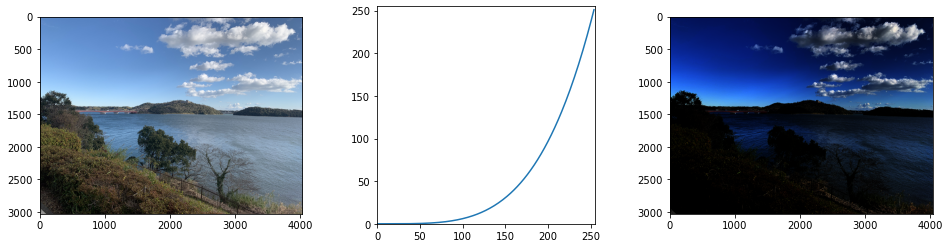
\includegraphics[scale=0.45]{kadai4_1_2.png}
    \end{center}
    \caption{$\gamma=\frac{1}{4}$の場合}
\end{figure}

\begin{figure}[h]
    \begin{center}
        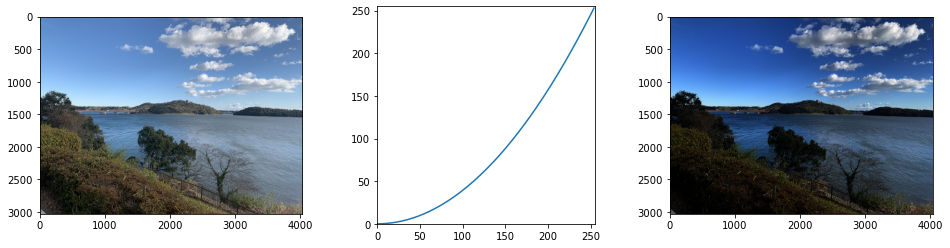
\includegraphics[scale=0.45]{kadai4_1_3.png}
    \end{center}
    \caption{$\gamma=\frac{1}{2}$の場合}
\end{figure}

\clearpage

\begin{figure}[h]
    \begin{center}
        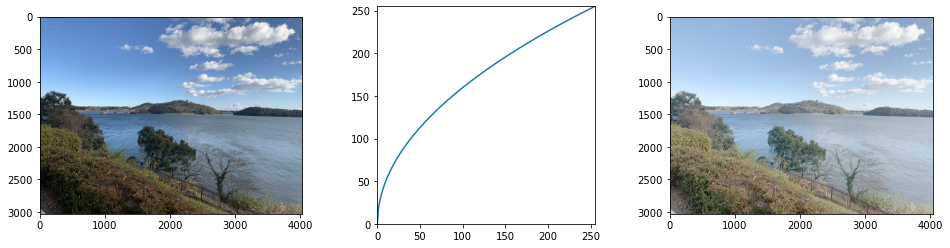
\includegraphics[scale=0.45]{kadai4_1_4.png}
    \end{center}
    \caption{$\gamma=2$の場合}
\end{figure}

また、作成するために用いたプログラムは付録のソースコード2に載せた。

\subsection{検討・考察}
実験の結果より、$\gamma$の値を1より小さくすることで全体が暗くなり、
$\gamma$の値を1より大きくすることで全体が明るい画像となった。

今回の画像に関しては元が明るい風景なので、
$\gamma$の値を図4のように明るくするのではなく、
図2,3のように暗くするほうが見た目が良いと考える。
$\gamma$の値を小さくしすぎると海の色が真っ黒になってあまり見えなくなるので
主観的に一番見た目が良いと思うものは$\gamma=\frac{1}{2}$(図3)である。

図3は、元の画像でぼんやりしている雲をくっきりしているので見た目が良くなっている。

\section{課題3}
\subsection{実験方法}
\subsection{実験結果}
\subsection{検討・考察}


\clearpage

\section{まとめ}



% 参考文献
\begin{thebibliography}{99}

\end{thebibliography}

\clearpage
\appendix
\section{付録}

\begin{lstlisting}[style = py,caption=kadai1]
    #4619055
    from skimage.io import imread, imsave
    import numpy as np
    import matplotlib.pyplot as plt
    plt.figure(figsize=(11,7))
    
    im1 = imread("data/Mandrill.bmp")  # カラー画像として読み込み
    im2 = imread("data/Mandrill.bmp")
    im3 = imread("data/Mandrill.bmp")
    
    for x in range(64,192):
        for y in range(25,220):
            im2[y,x] = np.dot(im2[y,x],[0.299, 0.587, 0.114])
    
    im3[25:220,64:192]= np.flipud(im3[25:220,64:192])
    
    plt.subplot(1, 3, 1)
    plt.imshow(im1)
    plt.title("original_Mandrill") 
    plt.subplot(1, 3, 2)
    plt.imshow(im2)
    plt.title("gray_Mandrill") 
    plt.subplot(1, 3, 3)
    plt.imshow(im3)
    plt.title("upside-down_Mandrill")
    plt.show()
\end{lstlisting}


\begin{lstlisting}[style = py,caption=kadai2]
    #4619055
    import numpy as np
    from skimage.io import imread, imsave
    from skimage.color import rgb2gray, gray2rgb
    import matplotlib.pyplot as plt
    %matplotlib inline
    
    def show_transform(im1, im2, h):
        """ 濃淡変換の入力画像,トーンカーブ,出力画像を描画
            im1 : 入力画像
            im2 : 出力画像
            h   : 階調変換関数
        """
        plt.figure(figsize=(16, 4))
        plt.subplot(1, 3, 1)
        plt.imshow(im1.astype(np.uint8), cmap="gray")
        
        plt.subplot(1, 3, 2)
        I = np.arange(0, 255)
        plt.xlim(0, 255); plt.ylim(0, 255); plt.gca().set_aspect(1.0)
        try:
            y = h(I)
            plt.plot(I, y)
        except:
            x = np.vstack([I, I, I])
            y = h(x.T)
            plt.plot(I, y[0,:,0], 'r', label='R')
            plt.plot(I, y[0,:,1], 'g', label='G')
            plt.plot(I, y[0,:,2], 'b', label='B')
            plt.legend()
       
        plt.subplot(1, 3, 3)
        plt.imshow(im2.astype(np.uint8), cmap="gray")
        
    def gamma(gam, I): return 255 * (I / 255) ** (1/gam)
    def gamma14(I): return gamma(1/4, I)
    def gamma12(I): return gamma(1/2, I)
    def gamma2(I): return gamma(2, I)
    
    f = imread("data/kadai2.jpg")
    
    show_transform(f, gamma14(f), gamma14)
    show_transform(f, gamma12(f), gamma12)
    show_transform(f, gamma2(f), gamma2)
\end{lstlisting}
%%%%%%%%%%%%%%%%%%%%%%%%%%%%%%%%%%%%%%%%%%%%%%%%%%%%%%%
\end{document}